%!TEX root = ../main.tex
\chapter{Krav}
Ud fra en opgaveformuleringen er der udarbejdet en rækker use cases som beskriver aktørernes interaktion med systemmet. Disse use cases er anvendt som karvaspecifikation, og er brugt som udgangspunkt til at fastlægge systemmet funktionalitet og design. De fulde use cases kan findes i dokumentationen under kravspecifikationen, sammen med de ikke fully dressed use cases, samt funktionelle krav. \newline


\begin{minipage}{0.45\textwidth}
\raggedright
\section{Aktørbeskrivelse}
I use casene ses en række aktører, der interagerer med systemet. Disse kan ses på aktørdiagrammet figur \ref{fig:actordiagram} og er beskrevet i den følgende aktørbeskrivelse. Flere detaljer om aktørene og hvordan de interagere med de ikke fully dressed use cases kan ses i projekt dokumentationen. 
\newline
\newline
\end{minipage}
\begin{minipage}{0.55\textwidth}
\begin{figure}[H]
	\centering
	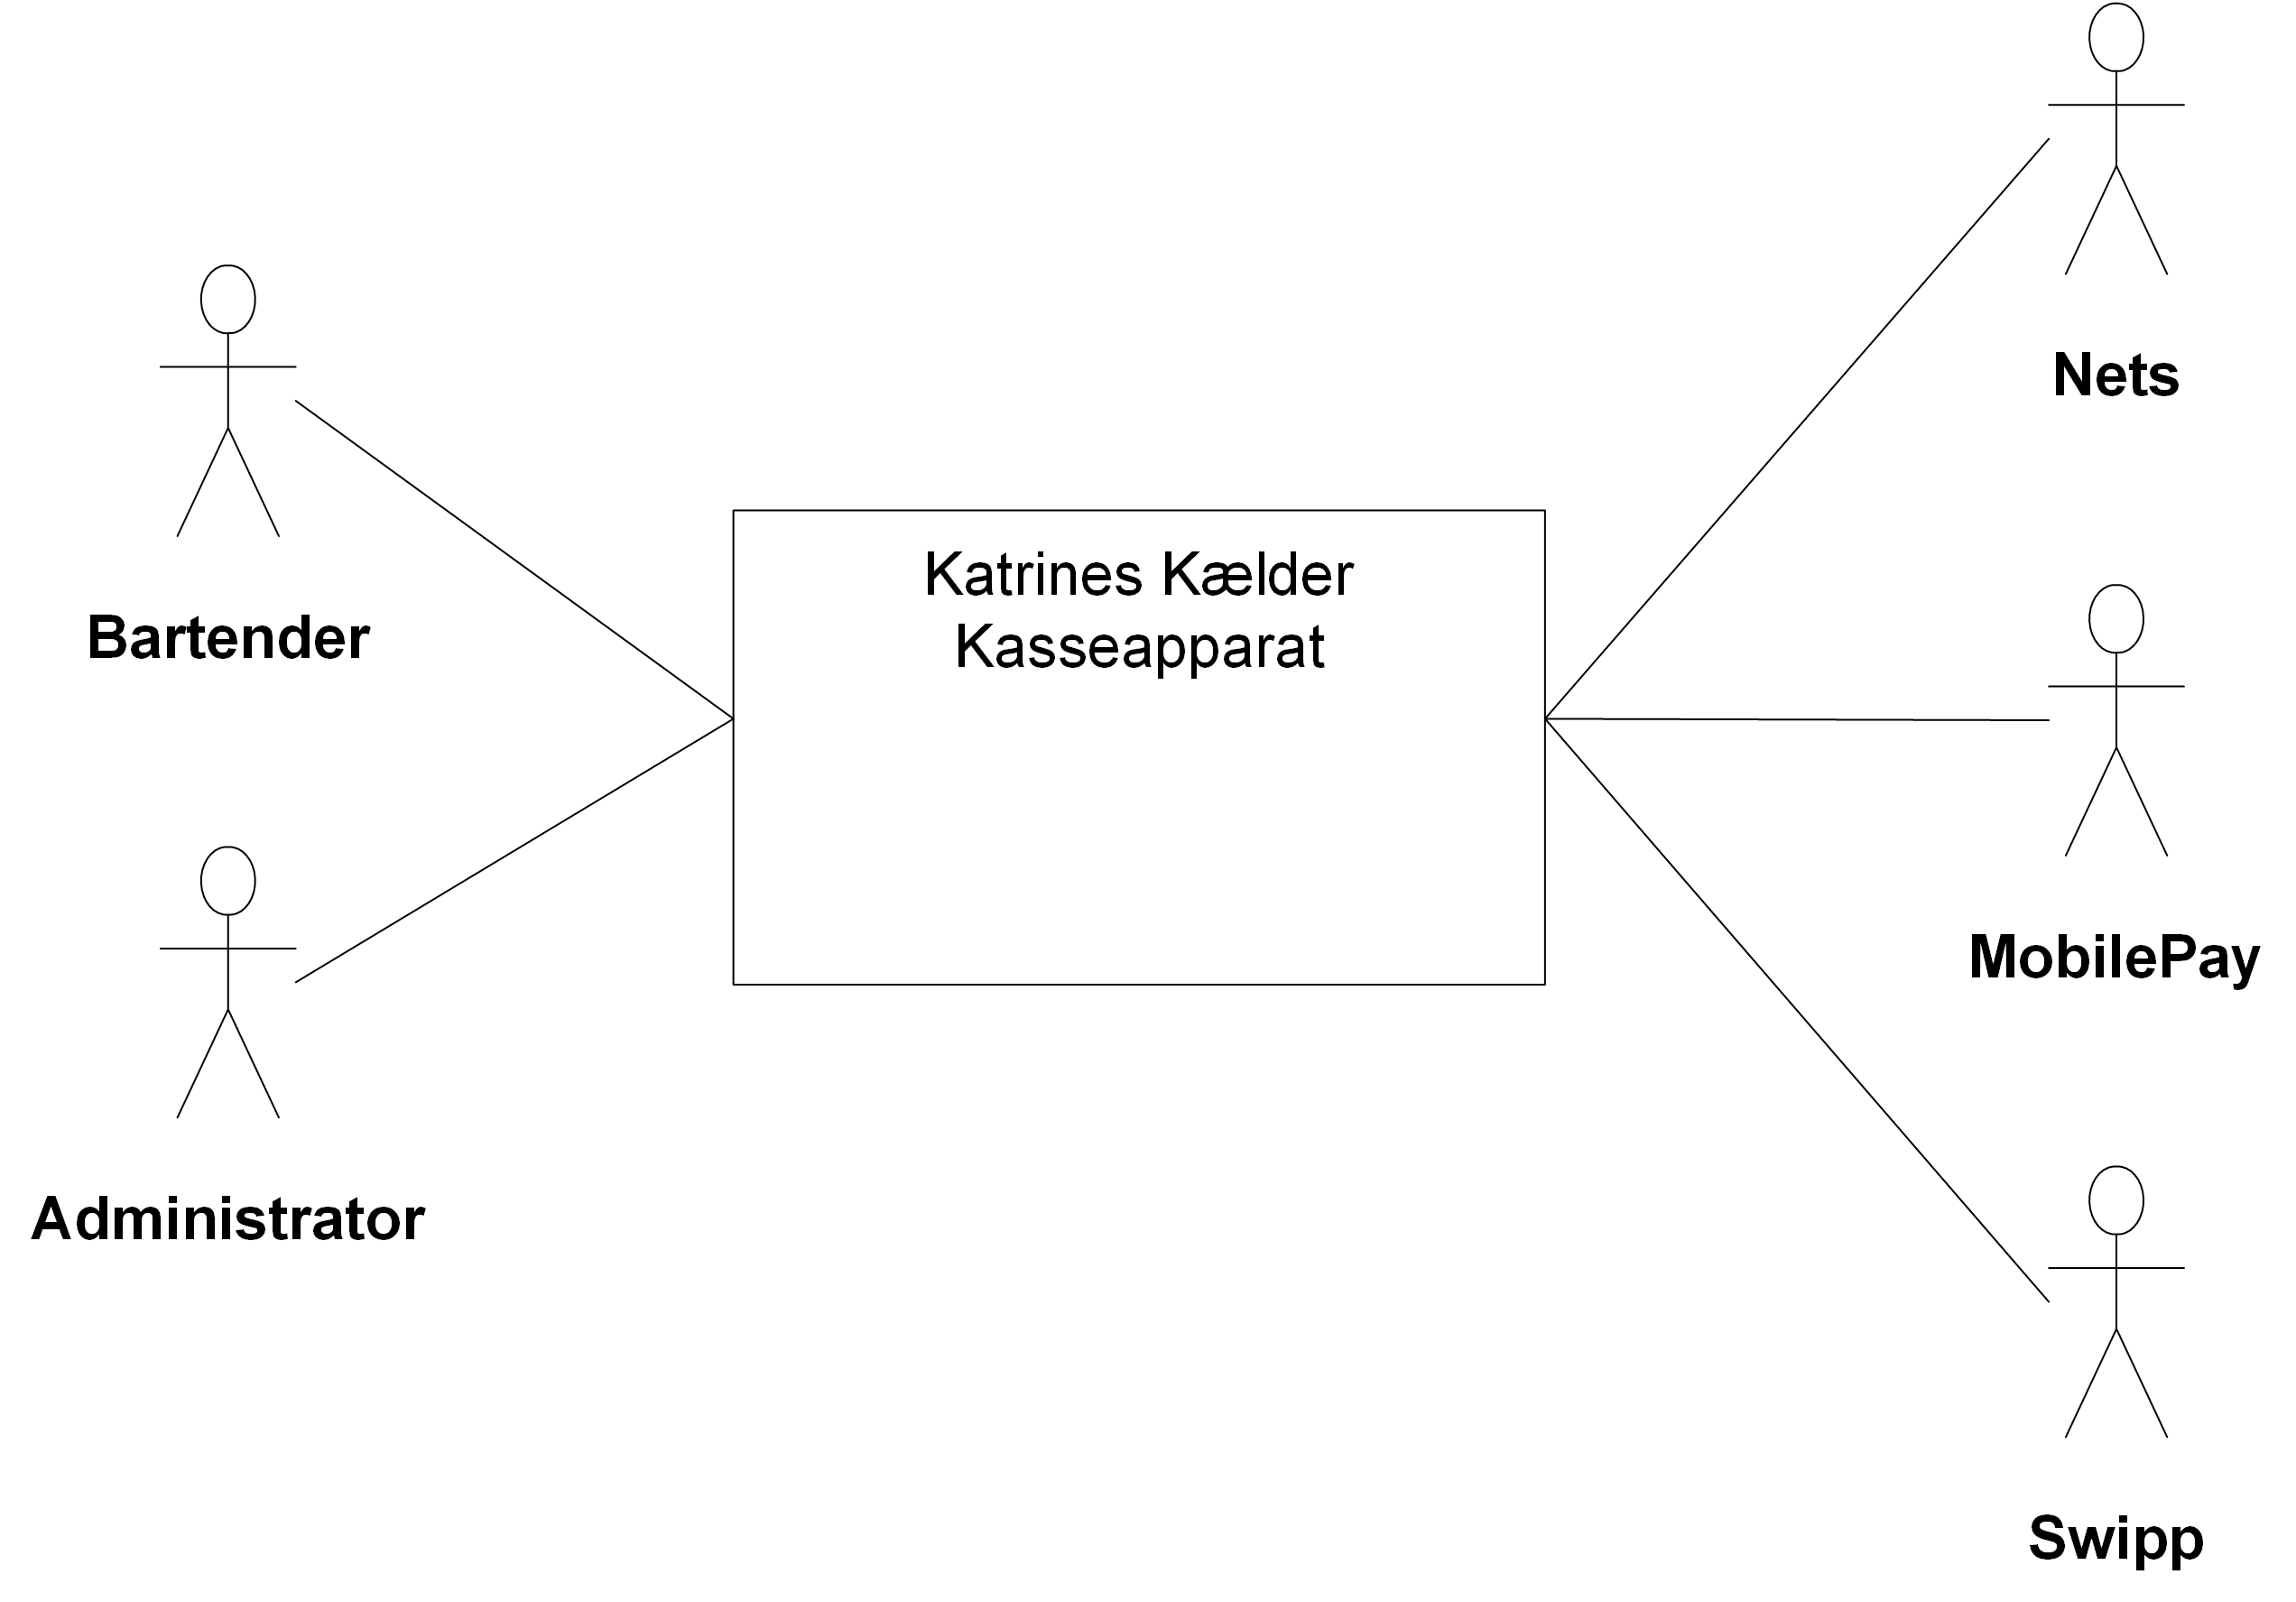
\includegraphics[width=0.7\textwidth]{Kravspecifikation/Actor/Actor.png}
	\caption{Aktør-kontekst diagram}
	\label{fig:actordiagram}
\end{figure}
\end{minipage} \hfill
\newline
\subsubsection*{Bartender}
er en primær aktør af systemmet, og står for salg af varer og betjening af systemmet. 

\subsubsection*{Admin}
er en primær aktør, som står for logistikken (priser, varer osv.) gennem systemmet. 

\subsubsection*{Nets}
er en sekundær aktør, som er leverandøren af betalingsterminalen. Betalingsløsningen er en af systemets primære betalingsløsninger.

\subsubsection*{MobilePay} 
er en sekundær aktør, det er en betalingsløsning som er leveret af Danske bank

\subsubsection*{Swipp} 
er en sekundær aktør, som er en betalingsløsning som leveres af Nordea, Nykredit, Sydbank, Jyske Bank, Arbejdernes Landsbank, Spar Nord Bank og Lokale Pengeinstitutter.  

\newpage

\section{Use Case beskrivelse}
De identificerede use cases er beskrevet i det følgende, her er der kun fokus på de fully dressed use cases. Hver use case beskriver et scenarie hvor aktører interagerer med systemet, hvor forholdet mellem de forskellige aktører kan ses på diagrammet figure \ref{fig:fullydressedusecases}

\begin{figure}[H]
	\centering
	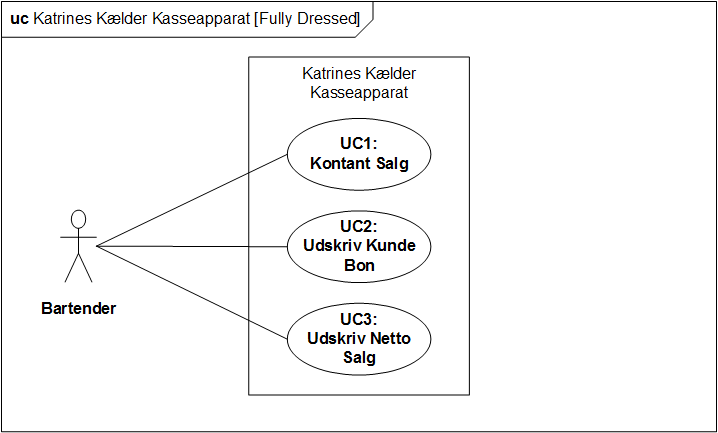
\includegraphics[width=0.6\textwidth]{Kravspecifikation/UseCases/UseCases_fully_dressed.png}
	\caption{Use-case diagram for de fully dressed use-cases.}
	\label{fig:fullydressedusecases}
\end{figure} 

\subsection*{Use Case 1: kontant Salg}
Bartenderen skal kunne sælge vare mod kontant betaling. Det sker ved at bartenderen trykke på de vare kunden ønsker og vælger kontant betaling på betalingssiden. 


\subsection*{Use Case 2: Udskriv Kundebon}
Hvis en kunde ønsker en bon skal en bartender kunne printe den ud. Det bliver gjort ved at vælge bon knappen som så udskriver en bon til kunden. 

\subsection*{Use Case 3: Kasseafstemning}
Når Det skal være muligt at printe en bon med hvor meget der er solgt for i løbet af aftenen, så bartenderen kan trykke på aftem knappen og printer en bon med samlede salg og dato udskrevet. 

\subsection*{Use Case 9: Tilføj vare til kasseapparat}
Det skal være muligt at tilføje flere vare til kasseapparatet. Det kan Admin gøre ved at gå ind under settings i WebApi og tilføje et product ved at udfylde felterne i Add Product og tryk submit. 

\subsection*{Use Case 10: Rediger vare i kasseapparat}
En vare skal kunne redigeres. Det gør Admin ved at gå ind på den vare som han ønsker at redigere under settings i WebApi. Her kan de ønskede værdier ændres og gemmes ved at trykke submit

\subsection*{Use Case 11: Fjern vare fra kasseapparat}
En vare skal kunne redigeres. Det gør Admin ved at gå ind på den var som han ønsker at slettet under settings i WebApi og trykke på Delete uden for varen.
